\subsubsection{DiseaseCore}

Darba autors jau projekta plānošanas stadijā zināja, ka vēlēsies padziļināti
izpētīt un apgūt \emph{multithreaded} aplikāciajs principus, tāpēc jau pašā sākumā
centās saprast, kur projektā varētu iesaistīt dažādu asinhrono un paralēlo darbību.

Šāda nepieciešamība noveda pie sekojošās koda arhitektūrās, kuras vispārīgo
vizuālo reprezentāciju var apskatīt \ref{img:multithreaded-layout} attēlā: visa plakne, kur tiks
veikta simulācija, tiek sadalīta vienādos apakšreģionos pa \(x\) asi (\emph{Region.cs}).
Katrā apakšreģionā atrodas kaut kāda noteiktu entītiju (gan veselo, gan slimo) apakškopa.
Katrs reģions tiek piešķirts noteiktai \emph{Task}\cite{csharp:task} instancei.
Tajā brīdī, kad noteiktais entītijs šķērso \(x\) ass robežu, tad tas tiek tiek
ievietots ,,Out of bounds" buferī, kuru regulāri apstrādā cita Task instance - šī instance
izvērtē katra entītija atrašanās vietu buferī un novieto to attiecīgā reģiona
,,inbound" buferī, kuru brīvā brīdī noteiktā \emph{Reģiona} Task pievienos
simulējamajiem entītijiem.


\begin{figure}[H]
	\centering
	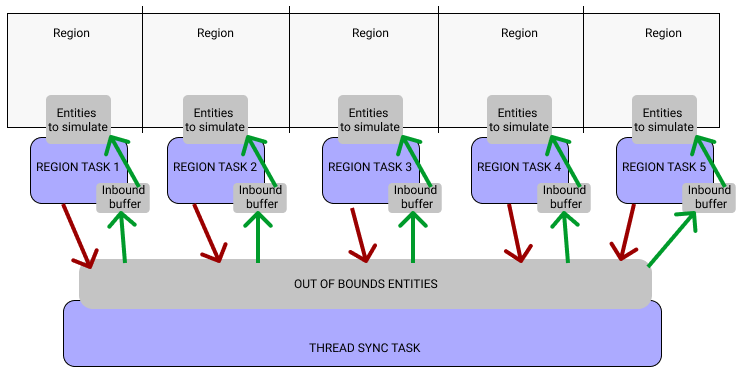
\includegraphics[scale=0.5]{images/multithreaded-layout.png}
	\caption{Reģionu sadalījums plaknei}
	\label{img:multithreaded-layout}
\end{figure}


Izvēle izveidot ,,inbound" buferi Reģioniem radās tādēļ, lai nerastos situācija,
ka entītiju simulācijas brīdī (kur tiek veikta iterēšana pār entītijiem) pēkšņi
rastos kaut kādas modifikācijas un \emph{undefined behaviour}.

Izvēle dalīt visu simulācijas laukumu reģionos pa \(x\) asi (varēja būt arī \(y\)
ass, tikai ne abas asis reizē), bija tāpēc, lai ērti varētu to pielāgot dažādu
kodolu skaitam -  sadalīt plakni \(n\) vienāda platuma un garuma daļās, lai
katram Reģionam būtu vienāds darbības laukums nepāra skaitļiem varētu rast zināmas problēmas.

Darba autors \textbf{neizmanto visus pieejamos procesora kodolus}, jo šādā gadījumā
procesors tiek pārslogots un netiek veikta responsīva UI updeitošanās (par to
vēlāk tiks aprakstīts) -- tāpēc tiek izmantota tiaki \(\frac{2}{3}\) no
pieejamajiem procesora kodoliem (vai sliktākajā gadījuma 1 kodols). Šī iemesla dēļ
\ref{img:multithreaded-layout} attēlā ir parādīti 5 reģioni/5 taski/ \(\frac{2}{3}\) no 8 kodolu sistēmas.

Lai gan, ņemot vērā, ka \(1 Task\neq 1 Thread\), jo Taski izpildās uz .NET Runtime
pieejama threadpoola\cite{csharp:tasks-not-threads}, tad reāli definēt vairāk
Tasksus arī ir iespējams -- runtime definētie threadi (mēdz saukt arī par
\emph{green threads}\cite{progr:green-threads}) izpildās
userspace\cite{sys:userspace}, nevis sistēmas kerneļa līmenī, kas .NET Runtime
atļauj pašam izlemt, kad darīt \emph{concurrent vai paralēlas}\cite{csharp:concurrent-parallel} darbības.
Tasku menedžošana
\emph{userspacā} ir daudz ātrāka nekā zemā līmeņa kerneļa threadu veidošana un izsaukšāna, atļaujot OS to menedžot.
Visi \emph{tasku} dalītie resursi tiek ,,aizsargāti" ar \emph{Mutex}\cite{csharp:mutex}
instancēm, kas garantē to, ka informācija (aizsargātais mainīgias) netiks vienlaicīgi lasīta/rakstīta no
vairākiem threadiem vienlaicīgi, datu integritāte tiek saglabāta. Izstrādes procesā
pareiza Mutex implementācija radīja daudzas kļūdas -- data races un deadlocks.

% CHAPTER LINQ un Pipeline


\subsubsection{frontendserver}

% Blazor UI kontrolē pipelines un instanciēšanu
% Notiek viss paralēlisms uz servera
% Canvas pakotne
% Data polling
